\section{La dinámica para la compuerta controlled-not}
La compuerta \textit{controlled not}, o CNOT, es el análogo cuántico de la compuerta lógica XOR. La compuerta XOR recibe como entrada dos bits, y arroja uno que puede ser $0$ si los bits de entrada tienen el mismo valor, o $1$ si tienen valores diferentes. Por otro lado, la compuerta cuántica CNOT actúa sobre un sistema de dos qubits, aplicando sobre el segundo qubit la compuerta $\sigma_{1}$ (NOT) si el primer qubit se halla en el estado $\ket{1}$, o dejándolo invariante si el primer qubit se halla en el estado $\ket{0}$. Esto es, cumple que \cite{Chuang}
\begin{align*}
    \ket{0}\otimes\ket{0}\mapsto\ket{0}\otimes\ket{0}\\
    \ket{0}\otimes\ket{1}\mapsto\ket{0}\otimes\ket{1}\\
    \ket{1}\otimes\ket{0}\mapsto\ket{1}\otimes\ket{1}\\
    \ket{1}\otimes\ket{1}\mapsto\ket{1}\otimes\ket{0} \rlap{.}
\end{align*}
En la base de los eigenestados de $\pauli{3}\otimes\pauli{3}$, la compuerta puede representarse como la matriz de permutación
\begin{equation*}
    \cnot=\begin{pmatrix}
        1&0&0&0\\
        0&1&0&0\\
        0&0&0&1\\
        0&0&1&0
    \end{pmatrix}.
\end{equation*}

Claro está, esta matriz corresponde a la evolución discreta. Para hallar la extensión a cualquier tiempo $t$, notamos que los eigenestados de este operador son $\ket{01}$, $\ket{00}$, $\ket{+}_{\cnot}$ y $\ket{-}_{\cnot}$ donde se definen
\begin{align*}
  \ket{+}_{\cnot}=\frac{\ket{10}+\ket{11}}{\sqrt{2}} & & \text{y} & & \ket{-}_{\cnot}=\frac{\ket{10}-\ket{11}}{\sqrt{2}}.
\end{align*}
Con esto es posible escribir la descomposición espectral del operador, y luego potenciarla 
\begin{align*}
\cnot=&P(\dyad{00}+\dyad{01}+\dyad{+}_{\cnot}-\dyad{-}_{\cnot})P^{\dag}\\
\Rightarrow \cnot^{t}=&P(\dyad{00}+\dyad{11}+\dyad{+}_{\cnot}+e^{i \pi t}\dyad{-}_{\cnot})P^{\dag}.
\end{align*}
La forma matricial del operador controlled not a un tiempo $t$ es análoga a la del operador SWAP:
\begin{equation}\label{eq:CNOT(t)}
\cnot^{t}=\begin{pmatrix}
  1 & 0 & 0 & 0 \\
  0 & 1 & 0 & 0 \\
  0 & 0 & e^{i\frac{t\pi}{2}}\cos{\frac{t\pi}{2}} & -ie^{i\frac{t\pi}{2}}\sin{\frac{t\pi}{2}}\\
  0 & 0 & -ie^{i\frac{t\pi}{2}}\sin{\frac{t\pi}{2}} & e^{i\frac{t\pi}{2}}\cos{\frac{t\pi}{2}}
 \end{pmatrix}
\end{equation}
Y esta es la cosa: esta definición del operador CNOT está bien, pero es muy arbitraria. Si trabajamos en la base de los eigenestados de $\pauli{1}$, CNOT también puede verse como un operador que voltea al qubit de control si el qubit objetivo está en el estado $\ket{+}$. Aún más lo de \textit{negar} qubits realmente solo tiene sentido cuando estos son puros y cuando se hallan en estados completamente alineados con el eje $z$ (si trabajamos en la base de $\pauli{3}$) o con el eje $x$ (si trabajamos en la base de $\pauli{1}$). En realidad, CNOT puede verse como una operación que induce un entrelazamiento entre las partículas siempre que el qubit de control no se halla completamente alineado con el eje $z$. La descripción del operador CNOT a través de una tabla de verdad es apegarse de forma innecesaria al paradigma del cómputo clásico. De ahí que me halla costado tanto trabajo trabajar con este operador.

El operador \textsc{CNOT} puede expandirse de la siguiente manera:
\begin{equation*}
        \cnot=\frac{1}{2}(\Id+\pauli{3}\otimes\Id+\Id\otimes\pauli{1}-\pauli{3}\otimes\pauli{1}).
\end{equation*}
Si se calcula el logaritmo de la compuerta es posible hallar el hamiltoniano generador de la unitaria,
\begin{equation*}
    H_{\cnot}=\frac{\pi}{4}\qty(\Id-\pauli{3}\otimes\Id-\Id\otimes\pauli{1}+\pauli{3}\otimes\pauli{1}),
\end{equation*}
que por ser una suma de operadores que conmutan entre sí, nos permite ver al controlled not como una aplicación consecutiva de tres unitarias diferentes
\begin{align*}
    \cnot&=e^{-i\frac{\pi}{4}\Id}e^{i\frac{\pi}{4}\pauli{3}\otimes\Id}e^{i\frac{\pi}{4}\Id\otimes\pauli{1}}e^{-i\frac{\pi}{4}\pauli{3}\otimes\pauli{1}}\\
    &=e^{-i\frac{\pi}{4}} (e^{i\frac{\pi}{4}\pauli{3}}\otimes \Id) (\Id \otimes e^{i\frac{\pi}{4}\pauli{1}}) e^{-i\frac{\pi}{4}\pauli{3}\otimes\pauli{1}}.
\end{align*}
Cuando se le expande en términos de productos tensoriales de operadores de Pauli, deja de ser claro el efecto clásico del CNOT, pero yo diría que esta es una mejor representación, porque está a un paso de expresarse en términos de compuertas de rotación y una de acoplamiento de Ising.
\subsection{CNOT completo efectivo}

Considérese el caso en que el aparato de medición no tiene un error asociado ($p=1$). En dicho caso, a través del principio de máxima entropía, se esperaría que el estado efectivo final fuera
\begin{equation*}
  \rho(t=1)=\rho(0)+\pauli{3}\rho(0)\pauli{3}=\frac{1}{2}(\Id+r_{3}\pauli{3}).
\end{equation*}


Este resultado viene del hecho que, en el caso $p=1$, el estado de máxima entropía es simplemente $\rho\otimes\frac{1}{2}$. ¿Por qué? Pues bien, con la interpretación de que CNOT aplica una compuerta $\pauli{3}$ sobre el qubit de control dependiendo del estado del qubit objetivo en la base de $\pauli{3}$, entonces se vuelve claro que si dicho qubit se halla en un estado completamente mezclado, el resultado será dicha mezcla: la mitad del tiempo se aplicará la compuerta, y la otra mitad, no (esto, claro está, cuando se toma la traza parcial, que ignora un montón de correlaciones y entrelazamientos que se forman durante el proceso).


Si se conociera la preparación microscópica del estado inicial, $\varrho$, el resultado de aplicar la compuerta de controlled not seguido de trazar al segundo sistema sería
\begin{equation*}
  \rho(t=1)=\frac{1}{2}\qty[\Tr_{1}(\varrho)+\pauli{3}\Tr_{1}(\varrho)\pauli{3}+\Tr(\pauli{1}\Tr_{2}(\varrho))(\Tr_{1}(\varrho)-\pauli{3}\Tr_{1}(\varrho)\pauli{3})]
\end{equation*}

Tanta traza marea, pero puede ser más claro si asumimos que al tiempo $t=0$ el sistema se halla en un estado separable $\varrho=\rho_{1}\otimes\rho_{2}$. En dicho caso es claro que la evolución está induciendo correlaciones entre ambos sistemas (correlaciones visibles únicamente en las compontentes $x$ e $y$ del primer subsistema), y que dicha correlación depende completamente de $\Tr(\sigma_{1}\rho_{2})$ (el valor esperado de la componente en $x$ del segundo susbsistema). De nuevo, como trazamos al segundo sistema, es más importante ver a este como el sistema de control, del que depende la acción sobre el sistema que nos interesa.

Para estudiar la dinámica efectiva del operador $\cnot$ son particularmente útiles las expresiones (\ref{eq:rhoArhoB}). Como el estado de máxima entropía compatible con la aplicación de grano grueso puede escribirse como $\varrho_{\max}=\rho_{A}\otimes\rho_{B}$, entonces hallar el estado efectivo final es un problema de álgebra, en efecto,
\begin{align*}
    \rho(t=1)=\frac{1}{2}[&p(\rho(0)+\sigma_{3}\rho_{A}\sigma_{3}+\Tr{\sigma_{1}\rho_{B}}[\rho_{A}-\sigma_{3}\rho_{A}\sigma_{3}])\\
    &+(1-p)(\rho(0)+\sigma_{1}\rho_{B}\sigma_{1}+\Tr{\sigma_{3}\rho_{A}}[\rho_{B}-\sigma_{1}\rho_{B}\sigma_{1}])].
\end{align*}
La estructura del estado final es una consecuencia directa de la aplicación borrosa. El primer término es el que vimos previamente, y el segundo es exactamente los mismo, pero para el que se han invertido los roles: es ahora el sistema que no nos interesa el que experimenta la acción del sistema de control.

En términos del vector de Bloch, que es una forma rápida de obtener el cambio de los observables y de la esfera, la dinámica se ve como
\begin{equation*}
    \vec{r}_{\rho}=(pr_{A}+(1-p)r_{B})\hat{r}_{\rho}\mapsto\begin{pmatrix}
        r_{B}(pr_{A}(\hat{r}_{\rho,1})^2+(1-p)\hat{r}_{\rho,1})\\
        r_{B}r_{A}(p\hat{r}_{\rho,1}\hat{r}_{\rho,2}+(1-p)\hat{r}_{\rho,2}\hat{r}_{\rho,3})\\
        r_{A}(p\hat{r}_{\rho,3}+(1-p)r_{A}(\hat{r}_{\rho,3})^{2})
    \end{pmatrix}.
  \end{equation*}
Lo que se observa es que las componentes $x$ e $y$ tienden a cero conforme $p$ tiende a uno. Las correlaciones que se generan sobre dichas componentes con un estado completamente mezclado se pierden (bajo la estimación de máxima entropía).

\subsection{CNOT efectivo a un tiempo arbitrario}

El CNOT efectivo a un tiempo arbitrario no me parece particularmente interesante, ahora que lo pienso. Pero puedo obtenerla sin mayor   problema. Ya tengo la expresión del CNOT para tiempos arbitrarios, después de todo.


  \begin{figure}[h!]
    \centering
    \begin{subfigure}{0.45\textwidth}
      \centering
      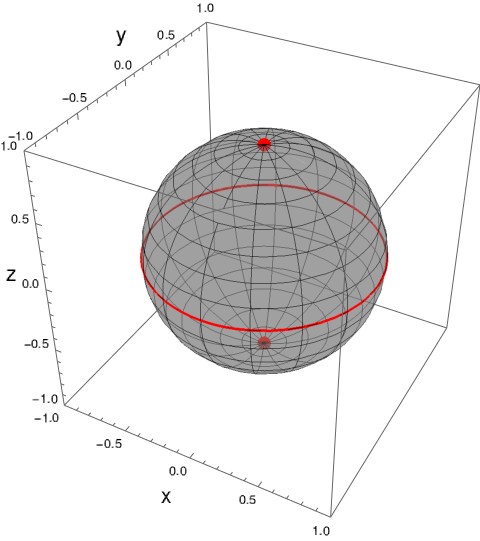
\includegraphics[width=0.9\linewidth]{maxent/figures/sphere_CNOT_t=0.0_z=0.8_p=0.95.png}
      \caption{$t=0$}
    \end{subfigure}%
    \begin{subfigure}{0.45\textwidth}
      \centering
      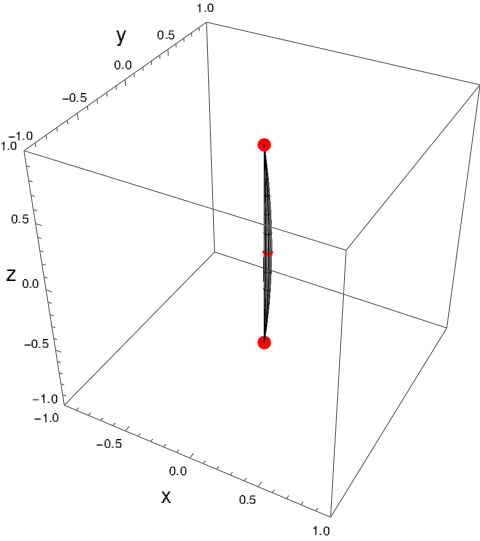
\includegraphics[width=0.9\linewidth]{maxent/figures/sphere_CNOT_t=1.0_z=0.8_p=0.95.png}
      \caption{$t=1.0$}
    \end{subfigure}
    \caption{Efecto de la evolución subyacente si $r=0.8$, $p=0.95$.}
    \label{fig:CNOTsequence2}
\end{figure}

\begin{figure}[h!]
    \centering
    \begin{subfigure}{0.45\textwidth}
      \centering
      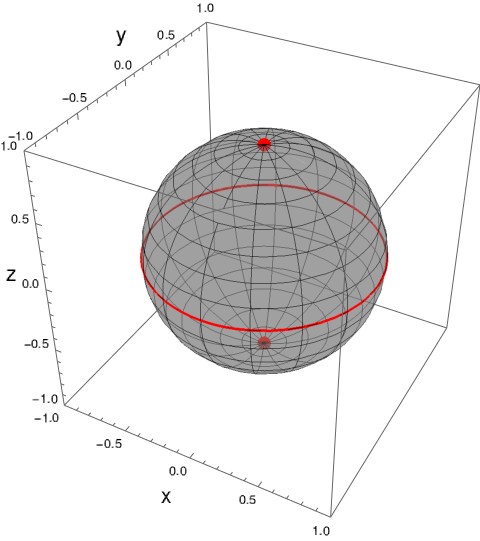
\includegraphics[width=0.9\linewidth]{maxent/figures/sphere_CNOT_t=0.0_z=0.8_p=0.6.png}
      \caption{$t=0$}
    \end{subfigure}%
    \begin{subfigure}{0.45\textwidth}
      \centering
      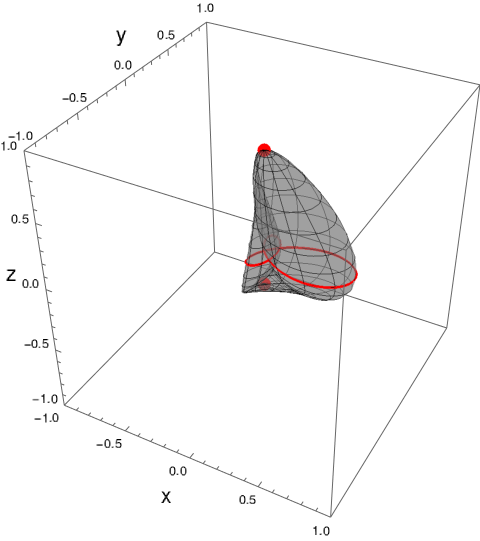
\includegraphics[width=0.9\linewidth]{maxent/figures/sphere_CNOT_t=1.0_z=0.8_p=0.6.png}
      \caption{$t=1.0$}
    \end{subfigure}
    \caption{Efecto de la evolución subyacente si $r=0.8$, $p=0.6$.}
    \label{fig:CNOTsequence2}
\end{figure}